% ---
% school: "college"
% level: "8eme"
% section: null
% chapter: "التناظر المركزي"
% source: "Axiomaths"
% title: "مناظرا رأسين وشبه منتصف"
% country: "Tunisie"
% year: 2026
% professor: "Axiomaths"
% difficulty: "Moyen"
% points: null
% tags: ["symetrie-centrale", "parallelogramme", "aire", "configuration"]
% ---
% Exercice 8/15 de la série 8ème « التناظر المركزي » (statement + \axsol + solution). Compiler avec XeLaTeX + axiomath.sty (+ axiomaths-logo.png).
\documentclass[12pt,a4paper]{article}
\usepackage[level=8b,color=15803D]{axiomath}
\usetikzlibrary{arrows.meta}
\newcommand{\cm}{\,\mathrm{cm}}
\axsetup{title={التناظر المركزي}, corrige}

\begin{document}

\begin{corr}[title={مناظرا رأسين وشبه منتصف}, stars=3, source={Axiomaths}]
$ABC$ مثلث، $E$ و $F$ مناظرتا $B$ و $C$ على التوالي بالنسبة إلى $A$ ، و $I$ منتصف $[BC]$.
\begin{center}
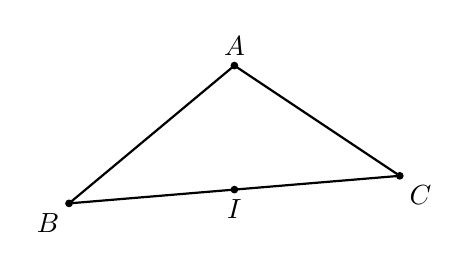
\begin{tikzpicture}[scale=0.7]
  \draw[thick] (0,0)--(6,0.5)--(3,2.5)--cycle;
  \fill (0,0) circle (2pt) node[below left] {$B$};
  \fill (6,0.5) circle (2pt) node[below right] {$C$};
  \fill (3,2.5) circle (2pt) node[above] {$A$};
  \fill (3,0.25) circle (2pt) node[below] {$I$};
\end{tikzpicture}
\end{center}
\begin{enumerate}
  \item ابنِ $E$ و $F$.
  \item بين أن $BCEF$ متوازي أضلاع.
  \item $J$ مناظرة $I$ بالنسبة إلى $A$. بين أن $J$ منتصف $[EF]$.
  \item بين أن مساحة $BCEF$ تساوي أربعة أضعاف مساحة $ABC$. \quad [لاحظ أن $A$ منتصف $[BE]$]
\end{enumerate}
\axsol
\begin{enumerate}[itemsep=14pt]
  \item $E$ على المستقيم $(BA)$ بحيث $A$ منتصف $[BE]$ ، و $F$ على $(CA)$ بحيث $A$ منتصف $[CF]$.
  \begin{center}
  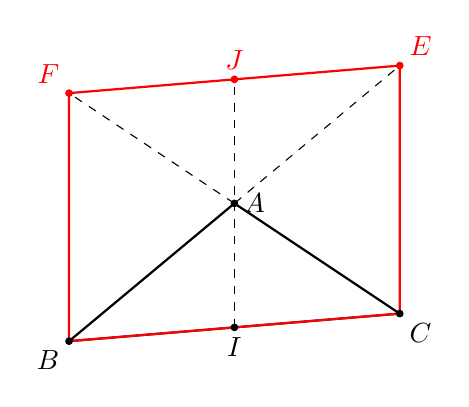
\begin{tikzpicture}[scale=0.7]
    \draw[thick] (0,0)--(6,0.5)--(3,2.5)--cycle;
    \draw[red,thick] (0,0)--(6,0.5)--(6,5)--(0,4.5)--cycle;
    \draw[dashed] (0,0)--(6,5);
    \draw[dashed] (6,0.5)--(0,4.5);
    \draw[dashed] (3,0.25)--(3,4.75);
    \fill (0,0) circle (2pt) node[below left] {$B$};
    \fill (6,0.5) circle (2pt) node[below right] {$C$};
    \fill (3,2.5) circle (2pt) node[right] {$A$};
    \fill (3,0.25) circle (2pt) node[below] {$I$};
    \fill[red] (6,5) circle (2pt) node[above right] {$E$};
    \fill[red] (0,4.5) circle (2pt) node[above left] {$F$};
    \fill[red] (3,4.75) circle (2pt) node[above] {$J$};
  \end{tikzpicture}
  \end{center}
  \item قطرا $BCEF$ هما $[BE]$ و $[CF]$ ؛ $A$ منتصف كل منهما (لأن $E=S_A(B)$ و $F=S_A(C)$). إذن $BCEF$ \ib{متوازي أضلاع}.
  \item التناظر $S_A$ يحوّل $B$ إلى $E$ و $C$ إلى $F$ ، فيحوّل $[BC]$ إلى $[EF]$ ، ويحوّل منتصف $[BC]$ (أي $I$) إلى منتصف $[EF]$. إذن مناظرة $I$ ، وهي $J$ ، منتصف $[EF]$.
  \item نقسّم $BCEF$ إلى أربعة مثلثات رؤوسها في $A$ : $ABC$ و $ACE$ و $AEF$ و $AFB$.
  \begin{itemize}
    \item $AEF$ مناظر $ABC$ ، و $AFB$ مناظر $ACE$ ؛ فمساحاتها متساوية مثنى مثنى.
    \item $ABC$ و $ACE$ لهما نفس الارتفاع المنطلق من $C$ ، وقاعدتاهما $AB=AE$ ، فلهما نفس المساحة.
  \end{itemize}
  إذن المثلثات الأربعة متساوية المساحة، ومنه :
  \[\ib{$\mathcal{A}(BCEF)=4\times\mathcal{A}(ABC)$}\]
\end{enumerate}
\textbf{الفكرة :} مركز التناظر يقسم متوازي الأضلاع إلى أربعة مثلثات متساوية المساحة.
\end{corr}

\end{document}
